\documentclass[11pt,a4paper]{article}
\usepackage[text={6.5in,10in},centering,a4paper]{geometry}
\usepackage{indentfirst}
\usepackage{setspace}
\usepackage{amssymb,amsmath} % Equations
\usepackage{tabularx} % Tables
\usepackage{graphicx,color} % Graphics, Figures
\usepackage[tight,footnotesize]{subfigure}
\usepackage{pgfgantt} % for gantt chart
\usepackage{hyperref}
\usepackage[nottoc,numbib]{tocbibind}
\usepackage[numbers]{natbib}

\graphicspath{{figures/}} % create a director 'figures' in your local dir and all pics are kept here

\renewcommand\familydefault{\sfdefault} % set to San Serif series

\begin{document}
\thispagestyle{empty}
\begin{center}
\doublespacing
{\Large \bf Senior Project Report 2102499}
\vfill
{
\Large \bf
% Project title
Solar Irradiance Forecasting for Chulalongkorn University Location Using Time Series Models
}
\vfill
{\Large \bf Justin Bieber Student ID XXXX} \\[2ex]
{\Large \bf Advisor: Assist. Prof. Jitkomut Songsiri}
\vfill
{\Large \bf Department of Electrical Engineering, Faculty of Engineering} \\[2ex]
{\Large \bf Chulalongkorn University} \\[2ex]
{\Large \bf Academic Year 20XX}
\end{center}

\newpage
\thispagestyle{empty}
\begin{center}
\textbf{Abstract}
\end{center}

This project considers a solar irradiance forecasting using time series models which finds an application in solar power prediction for energy management. The focuses of this project are on finding practical time series models for solar forecasting, proposing the effective approaches for missing-data and asynchronous sampled data issues, improving the models by removing seasonal trends from the historical data, and analyzing the effect of exogenous inputs which may be included in the models to improve the forecast. A time series prediction typically requires a complete set of historical data while the global horizontal irradiance (GHI) data in Thailand are frequently missing for consecutive days. This project proposes a data-missing imputation technique using the mean value of GHI averaged over the data corresponding to the same weather type. The required weather classification consists of two steps: a seasonal segmentation based on detecting changes of monotonic properties of temperature and humidity time series, and a nonlinear support vector machine (SVM) that uses weather labels from the previous seasonal segmentation. For asynchronous sampled data issue, the relevant variables in Thailand has the lower sampling rate than GHI. This project uses Spline interpolation to fill all data to be at the sampling rate. Autoregressive integrated moving average models (ARIMA) is considered in this project. To improve the accuracy, this project proposes two techniques for seasonal effect removal including Seasonal ARIMA models (SARIMA) and removal of seasonal trend fitted by Fourier Series. These models may be further improved if exogenous inputs are included in the models, known as ARIMA with Exogenous Variables (ARIMAX). Our studies found that other meteorological inputs which are relative humidity, air pressure, local temperature and wind speed marginally affect the accuracy of the forecast. At the end, we recommend to use SARIMA as the forecasting model based on a model selection criterion.

\paragraph{\textbf Keywords:} solar forecasting, ARIMAX models, Seasonal ARIMA, Fourier series, imputation (three to five)

\paragraph{\textbf Remark:}
\begin{enumerate}
\item The abstract should be fit in one page.
\item A report should not have more than 25 pages (exclude the cover, abstract, table of contents, acknowledgment, references, and appendices).
\end{enumerate}

This template is for preparing the senior project report in English. The guideline of writing the contents can be read from the Thai template.

\newpage
\thispagestyle{empty}
\tableofcontents

\newpage
\setcounter{page}{1}
\section{Introduction}

\subsection{Motivation}

\subsection{Objectives}

\subsection{Scope of work}

\subsection{Expected outcomes}

\subsection{Procedure}

\section{Methodology}

\section{Results and discussion}

\section{Conclusions}

\subsection{Summary}

\subsection{Problems and solutions}

\subsection{Suggestions}

\section{Acknowledgment}

\section{List of LaTeX usage}

\subsection{Tables}
\begin{table}[ht]
\centering
\caption{Example} 
\vspace{3mm}
\begin{tabular}{|l|c|c|r|} \hline
Item & Font & Font Type & Font Size \\ \hline
Title & Garamond & Bold & 20 \\
Author names & Garamond & Bold & 12 \\ 
Author affiliation/email & Garamond & Regular & 11 \\
Abstract/Keywords & Garamond & Regular & 11 \\
Level 1 headings & Garamond & Bold & 12 \\
Level 2 headings & Garamond & Bold & 11 \\
Level 3 headings & Garamond & Regular & 11 \\
Figure/table captions & Garamond & Regular & 11 \\
Main text/References & Garamond & Regular & 11 \\ \hline
\end{tabular}
\end{table}

\subsection{Figures}

\begin{figure}[ht]
	\begin{center}
		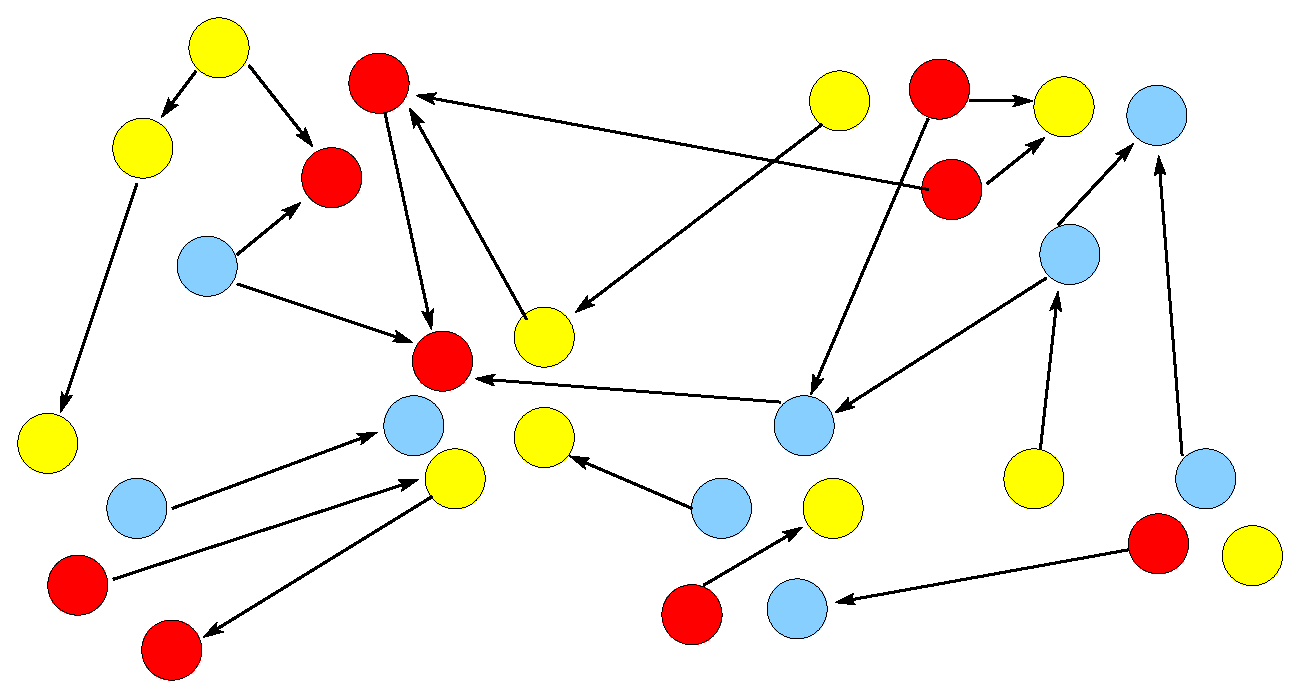
\includegraphics[width=0.7\linewidth]{gm.eps}
		\caption{Graphical model}
	\end{center}
\end{figure}

\begin{figure}[h!]
	\begin{center}
		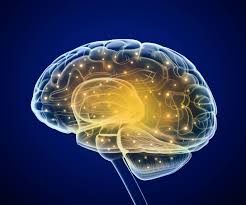
\includegraphics[width=0.5\linewidth]{brain.jpg}
		\caption{Brain impulses (Source: Shutterstock.com Image by: Alex Mit)}
	\end{center}
\end{figure}

\begin{figure}
\centering
\subfigure[first caption]{ 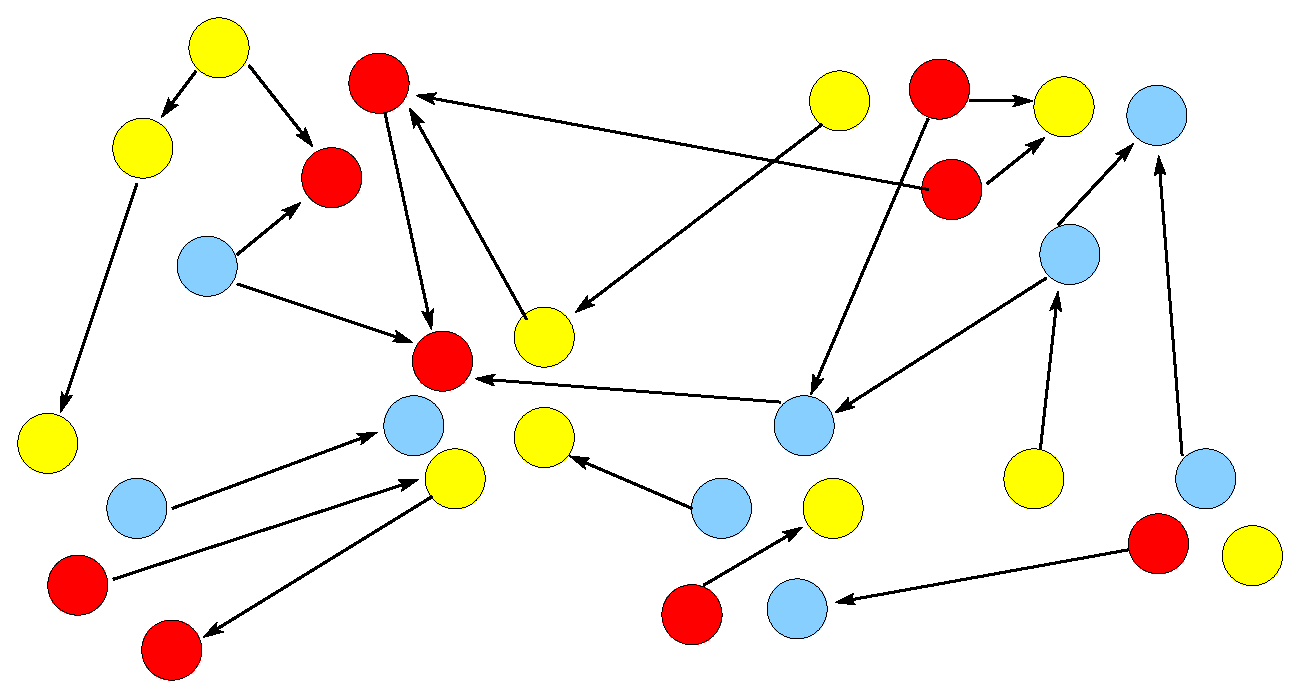
\includegraphics[width=0.45\linewidth]{gm.eps}  } 
\subfigure[second caption]{ 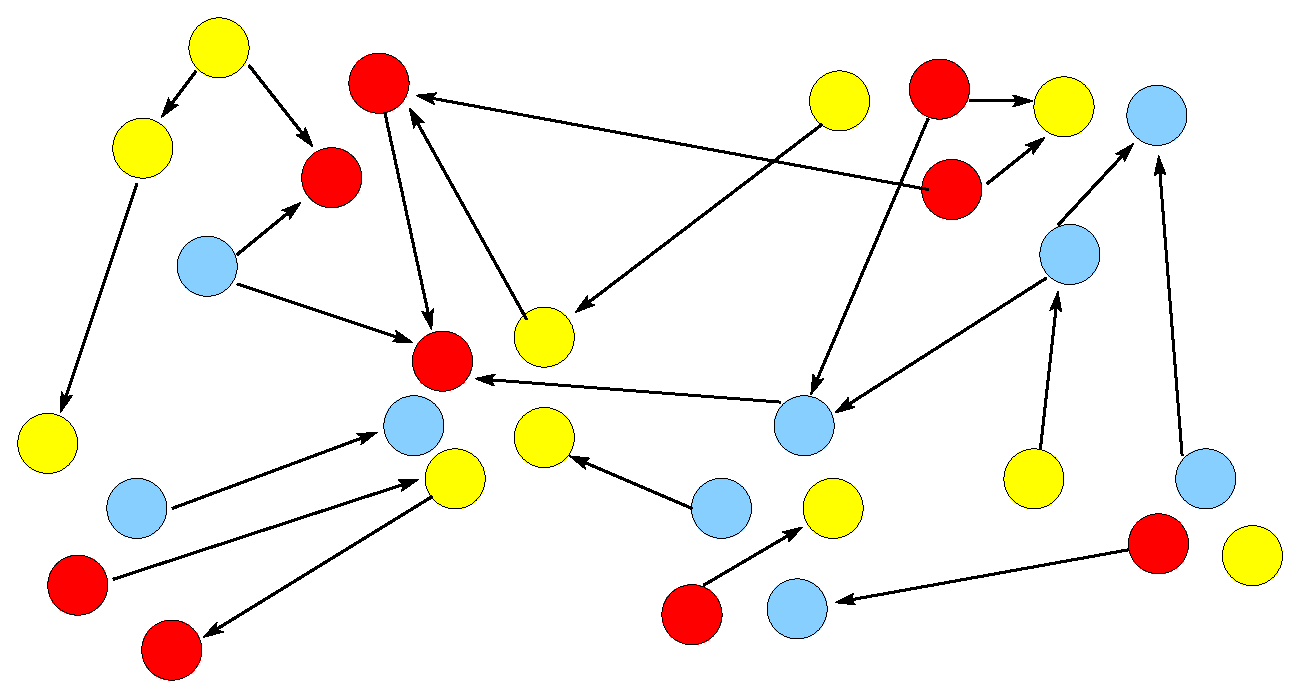
\includegraphics[width=0.45\linewidth]{gm.eps}  }
\caption{Subfigure example}
\end{figure}

\subsection{Equations}
$y=Cx$
\begin{equation}
	F(s) = \int_0^\infty e^{-st} f(t) dt
\end{equation}
the package 'align'
\begin{align}
    x    &= 2 \label{eq:x} \\
    y    &= 3 \label{eq:y} \\
    z    &= x \times y \nonumber \\
        &= p \label{eq:results}
\end{align}
\begin{itemize}
\item To not include an equation number, use \texttt{\nonumber} or \texttt{notag} 
\item Cross referencing can be done using \texttt{ref} or \texttt{eqref} together with \texttt{label}. For example, we refer to~\eqref{eq:x} that $x=2$.
\end{itemize}
the package 'eqnarray' is another environment to arrange equations into array format.
\begin{eqnarray}
\dot{x} &=& Ax + Bu \\
y &=& Cx+Du
\end{eqnarray}
If we want to align all equations into center use the package 'gather'.
\begin{gather}
y = \sum_{n=0}^100 0.5^n + \sin(2\pi n t) + \lim_{n \rightarrow \infty} \frac{\log n}{n} \\
z = \lim_{t \rightarrow \infty} e^{-st} g(t) 
\end{gather}

\subsection{References}
Reference formats are different from reference types. We commonly use the IEEE format, found in 

\url{https://ieee-dataport.org/sites/default/files/analysis/27/IEEE Citation Guidelines.pdf}

Use BibTex to generate reference list in the document. You will need a list of reference in the format of \texttt{file.bib} containing reference details, which can be exported easily using Google Scholar. When to refer to a paper, use \texttt{cite}. For example, the concept about system identification can be read from~\cite{SoS:89}. test \cite{CPM:89},\citep{CaA:15}, \cite{GrB:08b},\citep{JiY:09}

\bibliography{ref}
\bibliographystyle{ieeetr}

\section{Appendices}

\subsection{Appendix A}

\subsection{Appendix B}

\end{document}